\documentclass[10pt,letterpaper,unboxed,cm]{article}
\usepackage[margin=1in]{geometry}
\usepackage{graphicx}
\usepackage{enumerate} 
\usepackage{amssymb} 
\usepackage{amsmath}
\usepackage{fancyhdr}

\pagestyle{fancy}
\fancyhf{} 
\fancyhead[L]{CSE 105 Fall 2025}
\fancyhead[C]{Homework 1}
\fancyhead[R]{Due: Monday October 6 at 11:59pm}
\fancyfoot[L]{GROUP: James Villareal (A17450864), Tarun Upadhyay (A19113510), Kaitlyn Nguy (A19142421)}
\fancyfoot[R]{\thepage} 

\begin{document}

\begin{enumerate}

\item \textbf{Computation of a String on a DFA (Section 1)} \\
\emph{Question 1: Trace the computation on input $w = abba$. 
List the sequence of states visited (including start state) and state whether the input $w$ is accepted.} \\

\[
q_0 \xrightarrow{a} q_1 \xrightarrow{b} q_0 \xrightarrow{b} q_0 \xrightarrow{a} q_1
\]

The input $w$ is \textbf{not accepted} because the final state $q_1$ is not in $F$.

\item \textbf{Drawing a DFA (Section 2)} \\
\emph{Question 5: Draw a DFA over the alphabet $\{0,1\}$ that accepts all strings containing an even number of 0’s.}

\begin{figure}[h!]
    \centering
    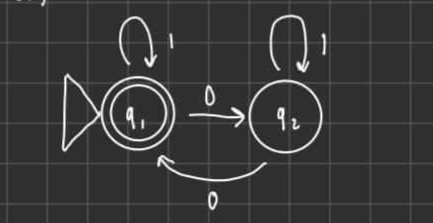
\includegraphics[width=0.75\linewidth]{images/cse105q5.png}
    \caption{DFA accepting strings with an even number of 0’s.}
\end{figure}

\item \textbf{Describing what a DFA does (Section 3)} \\
\emph{Question 9: Describe in words the set of strings accepted by $S$.
Give two examples of strings $S$ accepts and two it rejects.} \\

\textbf{Description:} The set of strings accepted by $S$ includes all strings over the described $\Sigma$ that end in \texttt{1}. \\[0.5em]
\textbf{Accepted Strings:} 01, 11 \\
\textbf{Rejected Strings:} $" "$, 10

\pagebreak

\item \textbf{Formal Definition of a DFA (Section 4)} \\
\emph{Question 13: Given the DFA below, write its 5-tuple $(Q, \Sigma, \delta, q_0, F)$ explicitly. Use a table to define $\delta$.} \\

\[
Q = \{q_1, q_2\}, \quad \Sigma = \{a,b\}, \quad q_0 = q_2, \quad F = \{q_1\}.
\]

\begin{center}
\begin{tabular}{||c||c c||}
\hline
$\delta$ & a & b \\
\hline\hline
$q_1$ & $q_1$ & $q_2$ \\
\hline
$q_2$ & $q_1$ & $q_2$ \\
\hline
\end{tabular}
\end{center}

\end{enumerate}

\end{document}